\chapter{Bitcoin Cash}
\label{cha:bch}

"Imagine you have a dollar in your wallet, and you put it aside for a while and 
then realize that one coin has split in two. Sounds weird? Not in the cryptocurrency 
world." That is an analogy with the fiat currency reported in an article of 
South China Morning Post\cite{scmp}.
Bitcoin is like a software, but, due to its distributed nature, unlike all the 
software we know, there is not a single entity which determines how it should be 
updated. As a result, in order to upgrade the blockchain it is necessary to be in 
agreement with the major part of the community. That is what happened on July 20$^{th}$,
2017, when the 97\% of the Bitcoin network voted to activate the "Segregated 
Witness" (SegWit) algorithm \ref{sec:segwit} to improve the scalability of Bitcoin. Although almost 
all the community agreed, some members believed that adopting SegWit without 
increasing the block size would simply postpone the scalability problem of Bitcoin.
As a result, on August 1$^{st}$, 2017 there were two forks of the Bitcoin network. 
One for adopting SegWit and one incrementing the size of the blocks giving 
birth to the Bitcoin Cash blockchain.\cite{scmp}\cite{thecryptonomist}

\section{Fork}
\label{sec:fork}

As said before, to have an upgrade in a blockchain we need the agreement of all
the network, otherwise those updates generates what is called a "fork". Basically, there are two types 
of fork:\medskip\\

\textbf{Soft Fork}
means that change in the blockchain protocol is backward-compatible. That means,
that although some nodes of the network are outdated, they are still able to 
process a transaction on the network, as long as they do not break the new protocol rules.
That is what happened with SegWit in August 2017.\medskip 
\begin{figure}
    \centering
    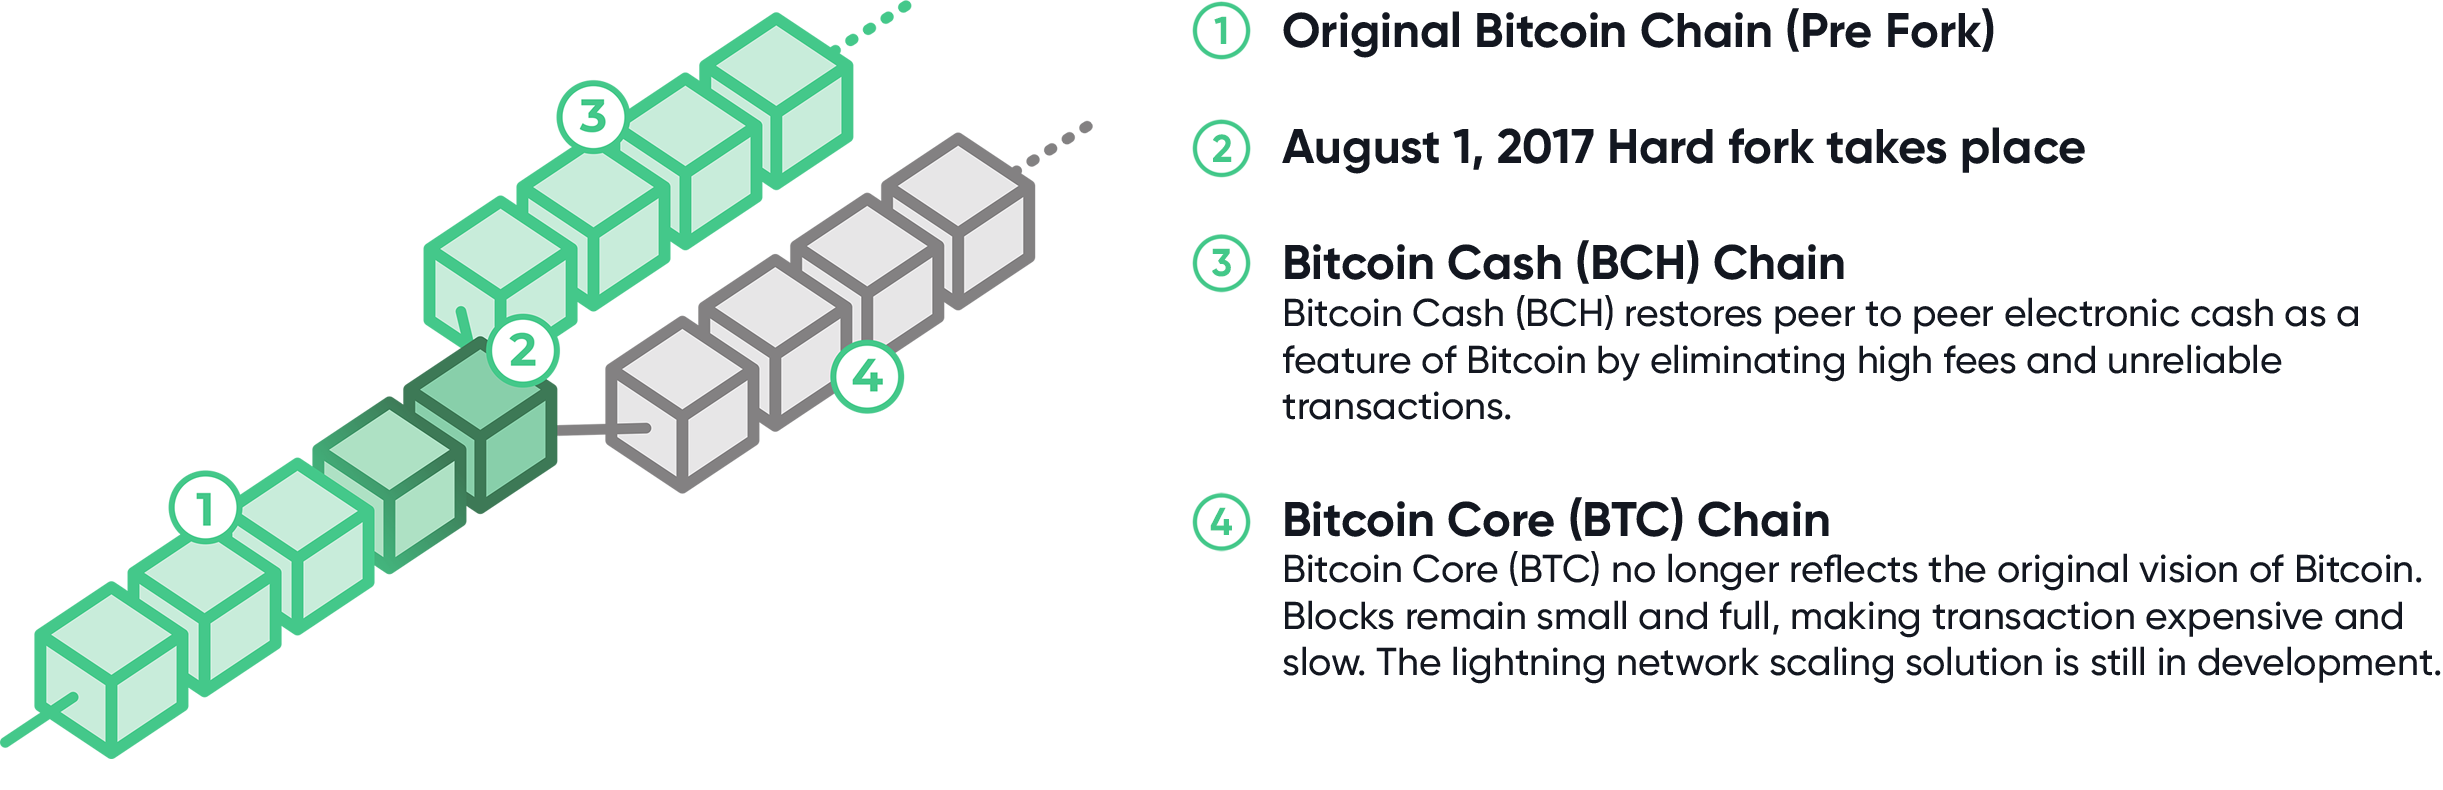
\includegraphics[height=5cm]{fork-img.png}
    \caption{A simple schema of the controversial hard fork of Bitcoin Cash. From \cite{bitcoin.com}}
    \label{fig:hardfork}
\end{figure}\\

\textbf{Hard Fork}
is the opposite. An obsolete node cannot perform any transaction on the new protocol.
According to the situation, a hard fork can either be planned or controversial.
In a planned fork, participants are going to upgrade their software voluntarily,
leaving the old version behind. The non-updated nodes are going to mine on the old 
blockchain, which will be used by very few participants.\\
In a controversial fork instead, there is a disagreement within the community about
the upgrade, so, the old blockchain is split into two new incompatible ones.\\ 
Both will have their own network, and as it happened to Bitcoin Cash on August 2017, 
will be developed in the way the participants believe is the best. This is where 
the analogy made at the beginning comes to help because, all the coins owned before 
the fork, will be split. So, the same amount of coins as before will be owned in 
both the blockchains.\cite{binancevision}\pagebreak


\subsection{SegWit}
\label{sec:segwit}

Segregated Witness is the major discrepancy between Bitcoin and Bitcoin Cash. In fact,
unlike BCH, where, to increase the number of transactions per second (TPS)
the block size was only incremented to 8 MegaByte, with SegWit the upgrade was more 
complicated. The transaction is split in two segments, the first, which is saved 
on the blockchain, contains the information about the sender and the receiver. 
Meanwhile, the second part containing the scripts and the signature of the sender remains at the 
bottom in a separate structure. As a result, the amount of information per transaction
is less and makes it possible to add more transactions in each block.\\
This is only one of the multiple benefits from the adoption of SegWit 
algorithm. To learn all about the benefits of this algorithm please read the official
documentation on the BitcoinCore website\cite{bitcoincore}.

\subsection{Addresses}
\label{sec:addresses}

Due to the nature of Bitcoin Cash, its addresses are generated in the exact same 
manner as the Bitcoin ones, so it is very difficult to recognize the source of 
a specific address. To facilitate its use and decrease the probability of being 
confused when someone tries to read it, the new Cashaddr Address 
Format was introduced. In a few words, it is only a new type of encoding which displays the 
address with a different pattern. Besides, every new Cashaddr corresponds to 
an old address, so when necessary, the outdated addresses can also be used.

\subsection{Block mining}
\label{sec:mining}

With the fork on August 1$^{st}$, 2017, Bitcoin Cash not only changed the block size but 
implemented also the "Emergency Difficulty Adjustment" (EDA) algorithm. The motivation was 
to have a method to convince miners to expend their resources in BCH. At the 
beginning, even the price of Bitcoin Cash was significantly lower than the price of 
Bitcoin, due to the fork process, the difficulty for mining was the same. So, it was 
less convenient to mine in the BCH blockchain. EDA resolved this problem by reducing 
the difficulty for block number $t$ by 20\% only when the time difference between the 
$(t-6)^{th}$ block and $(t-12)^{th}$ block had been greater than 12 hours. This system had been 
active from the 1$^{st}$ of August 2017, to the 12$^{th}$ of November 2017. Indeed, the next day, a hard fork
was made to implement the new "Difficulty Adjustment Algorithm" (DAA), which seeks to 
accomplish the following objectives:
\begin{itemize}
    \item Adjust difficulty to hash rate to target a mean block interval of 600 seconds.
    \item Avoid sudden changes in difficulty when the hash rate is fairly stable.
    \item Adjust difficulty rapidly when the hash rate changes rapidly.
    \item Avoid oscillations from feedback between hash rate and difficulty.
    \item Be resilient to attacks such as timestamp manipulation.
\end{itemize}
To fulfill all these requirements, the new algorithm adjusts the difficulty with each
block, taking into account the amount of work done and the elapsed time of the previous 
144 blocks.\cite{bitcoinabc}\cite{eda}\pagebreak
